% Capíulo 5
\chapter{Trabalhos Relacionados} \label{ch:trabalhos-relacionados}

Este capítulo confronta este trabalho contra outras pesquisas que analisam a evolução do desempenho de sistemas. Qualquer trabalho ou ferramenta que mensure a evolução do atributo de qualidade de desempenho e possua visualizações para exibi-la é considerado relacionado a este. Na seção \ref{sec:trabalhos-relacionados-ferramentas-profiling} são comentadas as ferramentas de \textit{profiling}. Na seção \ref{sec:trabalhos-relacionados-ferramentas-apm} são mostradas as ferramentas APM. Por fim, na seção \ref{sec:trabalhos-relacionados-adordagens-degradacao-desempenho} são exibidas as abordagens de medição da degradação de desempenho.

Muitas abordagens relacionadas a visualização de software têm sido propostas para comparar versões de software de um ponto de vista geral da arquitetura \cite{Steinbruckner2010b}\cite{Telea2008}\cite{Collberg2003}\cite{Eick1992}\cite{Holten2008}. Outras abordagens focam em visualizar as métricas do software em diferentes versões \cite{Langelier2008}\cite{Lanza2001}\cite{Pinzger2005}\cite{Wettel2008}. No entanto, essas abordagens diferem deste trabalho uma vez que o objetivo é comparar um aspecto dinâmico do software, o desempenho, ao invés de aspectos estáticos ou estruturais.

\section{Ferramentas de Profiling} \label{sec:trabalhos-relacionados-ferramentas-profiling}

Há ferramentas de \textit{profiling} que podem realizar a medição do atributo de qualidade de desempenho, no entanto, com diferentes características. O \textit{JProfiler} \cite{JProfiler} e o \textit{YourKit Java Profiler} \cite{Profiler2016} são ferramentas comerciais para realizar profiling de aplicações na linguagem Java. \citeauthor{SandovalAlcocer2013} comentam algumas limitações dessas duas ferramentas:
\begin{itemize}
	\item \textit{Variações de desempenho têm que ser manualmente rastreadas}: para cada execução, o \textit{profiler} tem que ser manualmente configurado para executar uma versão em particular. Depois, os dados do \textit{profiling} podem ser salvos no sistema de arquivos. Após realizar esse procedimento por duas vezes, ambas as execuções podem ser comparadas. Entretanto, cada execução requer muito trabalho manual;
	\item \textit{Faltam métricas relevantes}: ambas as ferramentas não consideram se o código-fonte foi alterado ou não. Como consequência, variações de desempenho em métodos não modificados podem distrair o programador de identificar alterações de código que realmente introduziram as variações;
	\item \textit{Representações visuais ineficientes}: O \textit{JProfiler} e o \textit{YourKit Java Profiler} usam uma tabela textual incrementada com alguns ícones para indicar variações. Dessa forma, entender qual variação de desempenho decorre de mudanças de software requer um esforço significativo do programador.
\end{itemize}

Os autores comentam que essas ferramentas, apesar de serem úteis para acompanhar o desempenho geral, são ineficientes para saber a diferença dos tempos dos métodos e, muitas vezes, insuficientes para compreender as razões para a variação de desempenho. Há ainda uma ferramenta que acompanha a JVM, chamada \textit{VisualVM}, que possui as mesmas limitações comentadas anteriormente. Além disso, o \textit{VisualVM} não oferece a comparação entre execuções, tornando difícil a visualização da evolução do desempenho entre as versões do software, uma vez que teria que ser feita manualmente para cada método desejado.

\section{Ferramentas APM} \label{sec:trabalhos-relacionados-ferramentas-apm}

O trabalho de \citeauthor{Ahmed2016} realizou um estudo para verificar se as ferramentas de gerenciamento de desempenho de aplicações - APM - são eficazes na identificação de regressões de desempenho. Os autores definem regressão de desempenho quando as atualizações em um software provocam uma degradação no seu desempenho. As ferramentas utilizadas no estudo foram \textit{New Relic} \cite{Relic2016}, \textit{AppDynamics} \cite{Appdynamics}, \textit{Dynatrace} \cite{Dynatrace2016} e \textit{Pinpoint} \cite{Pinpoint2016}. Como resultado, eles mostram que a maioria das regressões inseridas no código-fonte foram detectadas pelas ferramentas. Contudo, o processo de identificação do método exato cujo código foi inserido foi mais complicado, sendo necessário bastante trabalho manual: os autores inspecionavam as transações (requisições) marcadas como lentas e, manualmente, comparavam os respectivos \textit{stacktraces} para verificar se a ferramenta indicava corretamente a regressão de desempenho.

A ferramenta e a extensão proposta neste trabalho é diferente das ferramentas apresentadas no trabalho de \citeauthor{Ahmed2016} por realizar a análise de duas versões do software alvo do estudo, por automatizar o processo de identificação da causa do desvio de desempenho, por prover visualizações adequadas à identificação dos desvios de desempenho, bem como exibindo dados adicionais dos nós do grafo, por mostrar a evolução global e por cenário do desempenho e por proporcionar aos desenvolvedores a identificação diretamente do código-fonte das causas do desvio de desempenho.

\section{Abordagens de Degradação de Desempenho} \label{sec:trabalhos-relacionados-adordagens-degradacao-desempenho}

O trabalho de \citeauthor{SandovalAlcocer2013} propõe o \textit{Performance Evolution Blueprint}, uma abordagem visual para entender a causa de degradações de desempenho, comparando o desempenho de duas versões do sistema. Trata-se de uma visualização polimétrica, onde formas e cores dos elementos visuais indicam valores de métricas e propriedades do software analisado. O trabalho utiliza a ferramenta \textit{Rizel} para medição de propriedades dos métodos, tais quais: suas métricas, quais métodos foram adicionados, removidos ou modificados, e o seu tempo e número de execução. A abordagem foi desenvolvida na linguagem de programação Pharo. A Figura \ref{fig:trabalhos-relacionados-performance-evolution-blueprint} apresenta essa abordagem.

O trabalho proposto se diferencia do de \citeauthor{SandovalAlcocer2013} pelo fato de: (i) ser compatível com a linguagem Java; (ii) mostrar mais informações sobre a hierarquia de chamadas; (iii) exibir a evolução de cada cenário entre as versões do softwares; e (iv) utilizar diferentes elementos visuais para destacar a evolução do desempenho na visualização do \textit{call graph} dos cenários.

\begin{figure}[!htb]
   \centering
   \frame{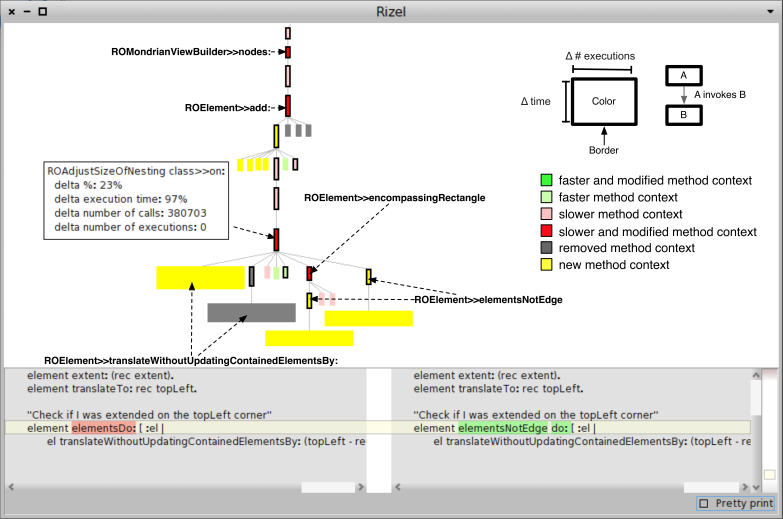
\includegraphics[scale=0.58]{Imagens/trabalho_relacionado_performance_evolution_blueprint.png}}
   \textsf{\caption[Exemplo do \textit{Performance Evolution Blueprint} \cite{SandovalAlcocer2013}]{Exemplo do \textit{Performance Evolution Blueprint} \cite{SandovalAlcocer2013}.\label{fig:trabalhos-relacionados-performance-evolution-blueprint}}}
\end{figure}

\citeauthor{Bergel} propôs uma abordagem cujo objetivo é comparar duas versões de um software. A visualização exibe informações de execução como um \textit{call graph}, onde os nós são os métodos e as arestas são as invocações. Cada nó é renderizado como uma caixa e uma invocação é uma linha que une dois nós. No entanto, essa abordagem considera apenas se um método gastou ou não mais tempo de execução do que na versão anterior. A Figura \ref{fig:trabalhos-relacionados-bergel-robbes-binder} exemplifica a visualização proposta pelos autores. O trabalho proposto se diferencia por adicionar mais métricas, como a porcentagem de desvio de desempenho dos métodos e se houve métodos adicionados ou removidos. Ainda, facilita a identificação da causa do desvio de desempenho, e irá prover aos desenvolvedores e arquitetos a possibilidade de verificar as mudanças no código-fonte ocorridas entre as duas versões comparadas.

\begin{figure}[!htb]
   \centering
   \frame{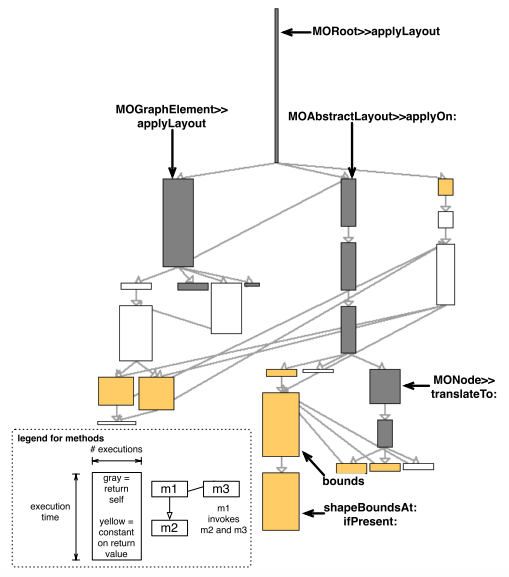
\includegraphics[scale=0.60]{Imagens/trabalho_relacionado_bergel_robbes_binder.png}}
   \textsf{\caption[Exemplo da visualização proposta por \citeauthor{Bergel}]{Exemplo da visualização proposta por \citeauthor{Bergel}.\label{fig:trabalhos-relacionados-bergel-robbes-binder}}}
\end{figure}

\citeauthor{Mostafa2009} propõem uma técnica que compara duas árvores de contexto de chamadas \abrv[CCT -- \textit{Context Call Tree}]{}(CCT, do inglês \textit{Context Call Tree}), cada uma obtida de uma versão diferente de um software. Os autores apresentam o \textit{PARCS}, uma ferramenta de análise que identifica automaticamente diferenças entre o comportamento da execução de duas revisões de uma aplicação. A abordagem usa como base o algoritmo de correspondência de árvores comuns para comparar duas CCTs. No entanto, o suporte visual usado pelo PARCS não representa adequadamente a variação de uma estrutura dinâmica e múltiplas métricas. Outra limitação dessa abordagem é que ela não detecta nós adicionados. Quando comparadas, duas CCTs que diferem apenas em um nó adicionado são consideradas completamente diferentes pelo PARCS. A Figura \ref{fig:trabalhos-relacionados-parcs} exibe um exemplo dessa abordagem. O trabalho proposto detecta e representa visualmente nós adicionados e removidos, uma vez que é fundamental para o entendimento do real impacto no desempenho de determinada árvore de chamadas, além de apresentar métricas como a variação de desempenho, o tempo de execução e a quantidade de execuções dos nós.

\begin{figure}[!htb]
   \centering
   \frame{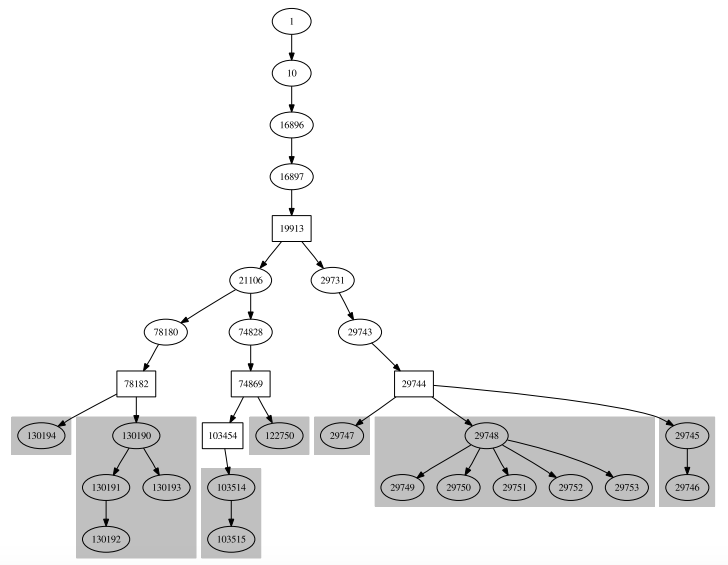
\includegraphics[scale=0.60]{Imagens/trabalho_relacionado_parcs.png}}
   \textsf{\caption[Exemplo do PARCS \cite{Mostafa2009}.]{Exemplo do PARCS \cite{Mostafa2009}.\label{fig:trabalhos-relacionados-parcs}}}
\end{figure}

\citeauthor{Bezemer2015} realizam a comparação do desempenho de duas versões de um software através de gráficos de chama diferenciais (do inglês, \textit{differential flame graphs} -- DFG). Dadas duas versões v1 (anterior) e v2 (atual), a ferramenta realiza a comparação de três maneiras: (i) com v1 como base, (ii) com v2 como base e (iii) apenas as diferenças do item (ii). Utiliza cores para destacar as comparações: o branco indica que não houve mudanças, o azul que houve melhora no desempenho e o vermelho indica que este piorou. Entretanto, a abordagem não indica as causas das variações de desempenho e os autores indicam que o principal desafio é a coleta dos dados, pois são necessárias ferramentas de \textit{profiling} de terceiros para a análise das versões e eles destacam que pode ser difícil coletar os dados para algumas linguagens, como o Java e Python. A Figura \ref{fig:trabalhos-relacionados-dfg} mostra o DFG. O \textit{\toolName}, para cada método com variação de desempenho, identifica as possíveis causas dessas variações e apresenta os \textit{hashs} dos \textit{commits} que representam essas modificações.

\begin{figure}[!htb]
   \centering
   \frame{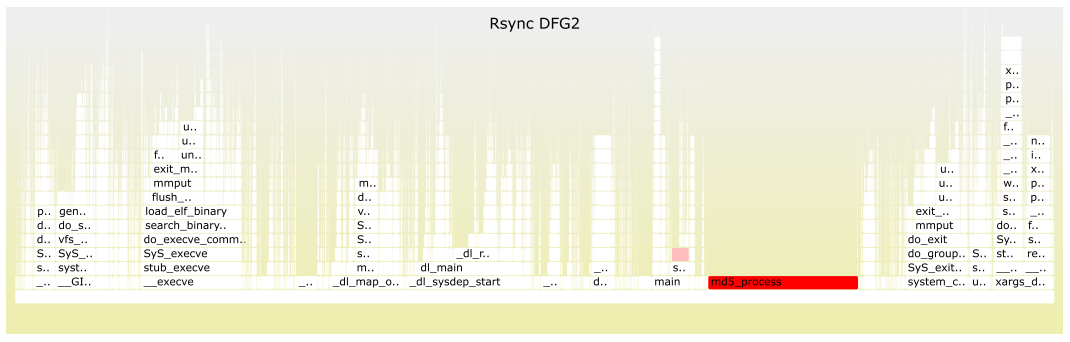
\includegraphics[scale=0.42]{Imagens/trabalho_relacionado_dfg.png}}
   \textsf{\caption[Exemplo do DFG \cite{Bezemer2015}.]{Exemplo do DFG \cite{Bezemer2015}.\label{fig:trabalhos-relacionados-dfg}}}
\end{figure}